\documentclass{scrartcl}

% Kodierung dieser Datei angeben
\usepackage[utf8]{inputenc}

% Schönere Schriftart laden
\usepackage[T1]{fontenc}
\usepackage{lmodern}

% Deutsche Silbentrennung verwenden
\usepackage[ngerman]{babel}

% Anführungszeichen mit \enquote
\usepackage{csquotes}

\usepackage{amsmath}

 \usepackage{amsthm}


% Bessere Unterstützung für PDF-Features
\usepackage[breaklinks=true]{hyperref}

\KOMAoptions{%
  % Absätze durch Abstände
  parskip=full,%
  % Satzspiegel berechnen lassen
  DIV=calc%
}

% TikZ laden
\usepackage{tikz}

% Verwendete TikZ-Bibliotheken laden
\usetikzlibrary{positioning,automata}

\begin{document}
\tableofcontents
\begin{tikzpicture}[auto, thick]
 \node[initial, state] (q0) {$q_0$};
 \node[state, right=of q0] (q1) {$q_1$};
 \node[state, accepting, right=of q1]
 (q2) {$q_2$};
 \path (q0) edge[->] node {0} (q1)
 (q1) edge[->, loop above] node {0} ()
 edge[->, bend left] node {1} (q2)
 (q2) edge[->, bend left] node {0} (q1);
\end{tikzpicture}

\section{Kapitel}
test zeilenumbruch\\
testende

Wir setzen \(a^{n_{L}}b^{n_{L}}\in L \) mit \(|z|=2n_{L}\leq n_L\). Also existiert eine Zerlegung \(z=uvw\) mit




% \nopunct und [] zum �ndern der �berschrift
  \begin{proof}[\nopunct]
  %\tag f�r Beschriftung der Formel
  \begin{align*}
    \intertext{Bew:}
      S &\Rightarrow^* a^nAb^nc^n \tag{IV}\\
      &\Rightarrow^* a^nb^nAc^n \tag{n-mal 14}\\
      &\Rightarrow a^nb^nBbccc^{n-1} \tag{15}\\
      &\Rightarrow^* a^nBb^{n+1}c^{n+1} \tag{n-mal 16}\\
      &\Rightarrow a^{n+1}b^{n+1}c^{n+1}\in \text{L(G)} \tag{17}\\
      \intertext{oder:}
      &\Rightarrow a^{n+1}Ab^{n+1}c^{n+1}\in \text{L(G)} \tag{18}
  \end{align*}
  \end{proof}


\begin{enumerate}
  \item\(|uv|\leq n_L\)
\end{enumerate}


\textbf{test zeilenumbruch}sds

testende
\textsc{Packungen}.
\enquote{Packungen}

\subsection{Subsection}
\begin{enumerate}
 \item
       ctrl+shift +7 für Auskommentieren an/aus
 \item
       \(\$\$\) für displaymath und nur eins für inlinemath
 \item
       ctrl+alt+7 für \(\{\}\) um Markierung
 \item
       \ref{tbl:einwohner}testref

       \begin{figure}
        \begin{center}
         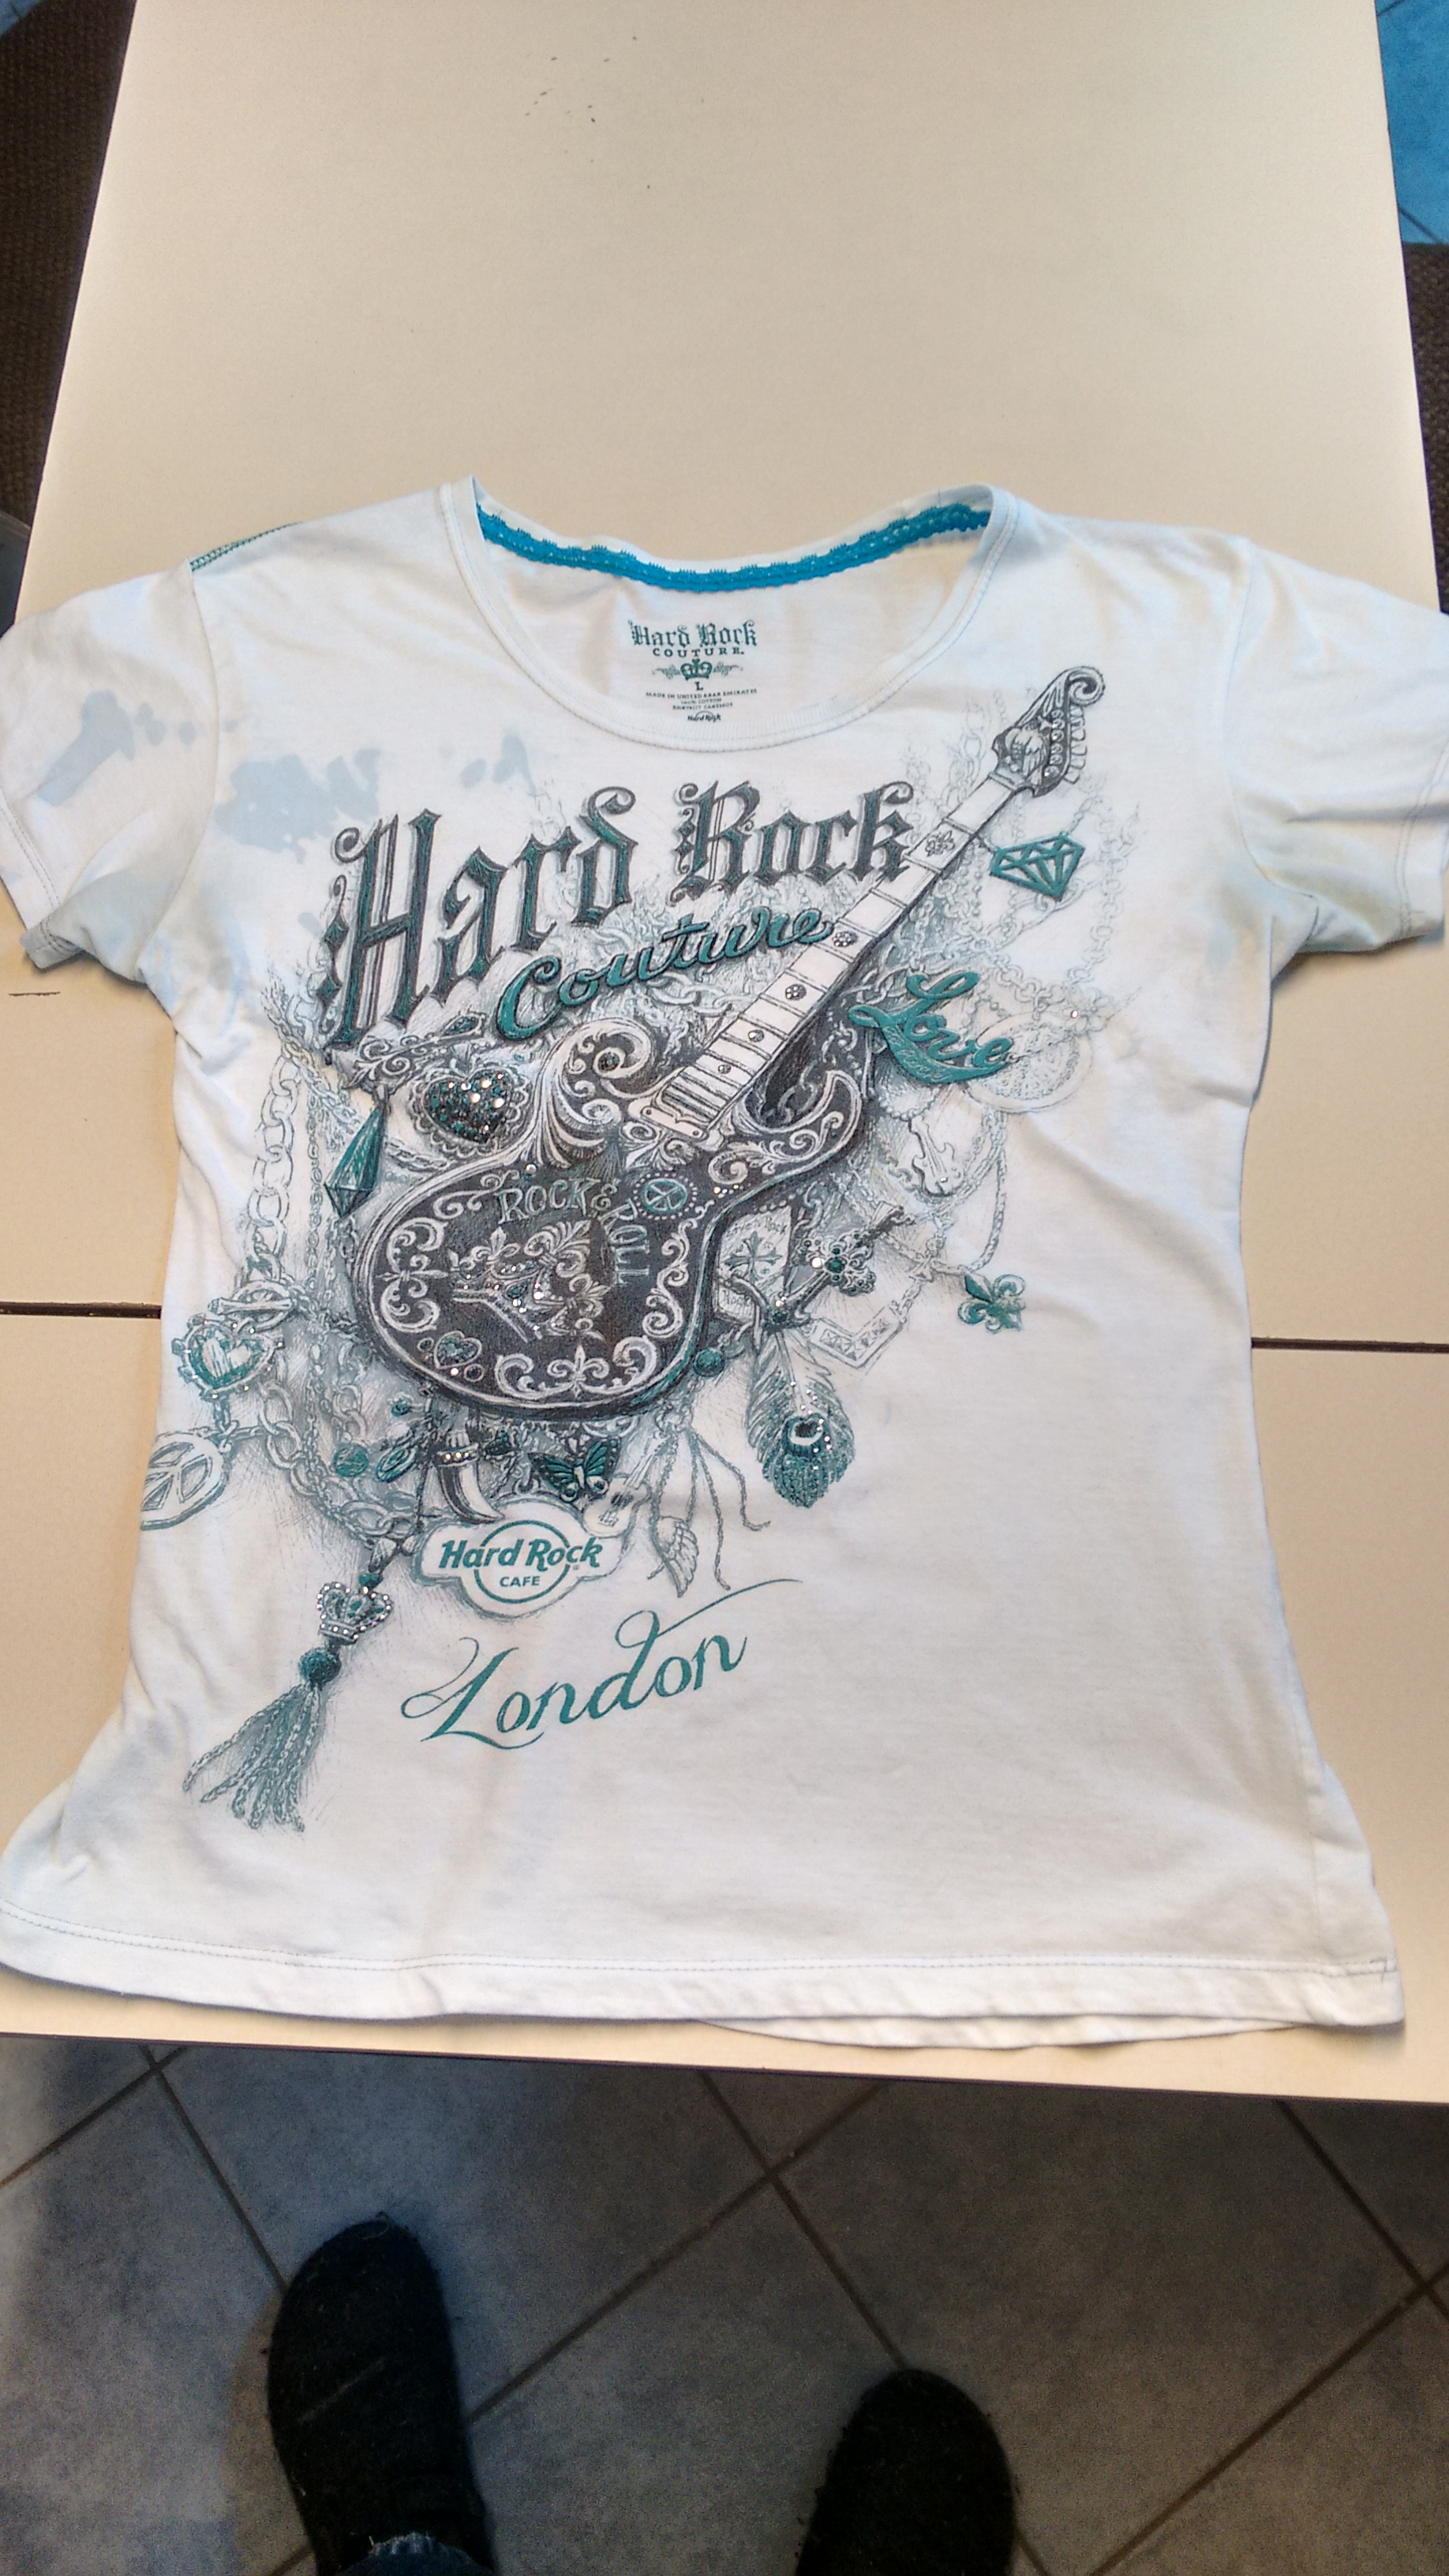
\includegraphics[width=4cm]{testbild.jpg}
        \end{center}
        \caption{T-shirt}
        \label{fig: tshirt}
       \end{figure}



\end{enumerate}

\begin{description}
 \item[Gummibär] gummi
 \item[ich] person
\end{description}
\subsubsection{Subsub}
% h als option steht für die Positon wo es definiert wurde
\begin{table}[h]
 \centering
 \begin{tabular}{l|ll}
  \textbf{Jahr} & \textbf{D} & \textbf{F}
  \\  \hline
  1990          & 34         & 54         \\
  2000          & 64         & 89
 \end{tabular}
 \caption{Jahreszahlen}
 \label{tbl:einwohner}
\end{table}

\end{document}
